% !TeX root = ..//fp_nmr_schmitt_kleinbek_18.tex

\thispagestyle{empty}
\frame{\titlepage}
\frame{\frametitle{Inhaltsübersicht}\tableofcontents}


%---------------
%Relaxationszeiten
%---------------
\section{Relaxationszeit}
\begin{frame}{Physikalischer Hintergrund}
	\begin{itemize}
	\item Teilchen mit Spin $S\neq 0$ befindet sich in externem Feld $\vec{B_{0}}$
	\item Dipolmoment
		\begin{align*}
		\vec{\mu}=\hbar\gamma\cdot\vec{S}
		\end{align*}
	\item Energieaufspaltung durch parallele bzw. antiparallele Ausrichtung
		\begin{align*}
		\Delta E = -\vec{\mu}\cdot\vec{B}_0
		\end{align*}
	\item Ungleichmäßige Besetzung der anti-/parallelen Zustände (Fermi-Dirac Verteilung)
		$\Rightarrow$ Boltzmann Näherung
		\begin{align*}
		\frac{N_+}{N_-}=\e{\frac{2\Delta E}{\k_\text{b} T}}
		\end{align*}
	 \item Magnetisierung 
		\begin{align*}
		\vec{M}=\frac{1}{V}(N_+-N_-)|\vec{\mu}|\vec{e_{z}}
		\end{align*}
	\end{itemize}
\end{frame}

\begin{frame}{Physikalischer Hintergrund}
	\begin{itemize}
	\item Drehmoment $\vec{\tau}=\vec{M}\times\vec{B}_0$
	\item Differentialgleichung $\dv{\vec{M}_\bot}{t}=-\gamma\vec{M}_\bot\times\vec{B}_0$
	\end{itemize}
	\begin{block}{Rotation mit Larmorfrequenz}
		\[
		\omega_\text{L}=\gamma B_0
		\]
	\end{block}
	\begin{figure}
	% !TeX root = ..//f61_longreport_schmitt_kleinbek.tex
\begin{tikzpicture}[scale=.75]
\draw[arrows=-{Stealth[scale=.75]}, ultra thick, color=grey] (0,0)--+(0,4) node [above]{$B_0$};
\draw[arrows=-{Stealth[scale=.75]}, line width=1mm, color=myred] (0,0)--+(0,2) node [left]{$M$};
\fill (0,0) circle (1.9pt)[color=myred];

\draw [thick, rotate=-23](3.7,3.43) ellipse (.8cm and .4cm);
\draw[arrows=-{Stealth[scale=.75]}, ultra thick, color=grey] (4,0)--+(0,4) node [above]{$B_0$};
\draw[arrows=-{Stealth[scale=.75]}, ultra thick, color=grey, dashed] (4,0)--+(1.5,0) node [below]{$B_1$};
\draw[arrows=-{Stealth[scale=.75]}, line width=.75mm] (4,0)--+(1.5,4) node [right]{$B_\text{tot}$};
\draw[arrows=-{Stealth[scale=.75]}, line width=1mm, color=myred] (4,0)--+(0,2) node [left]{$M$};
\fill (4,0) circle (1.9pt)[color=myred];

\draw [thick, rotate=18](11.3,-2.8) ellipse (1.9cm and .4cm);
\draw[arrows=-{Stealth[scale=.75]}, ultra thick, color=grey] (12,0)--+(0,4) node [above]{$B_0$};
\draw[arrows=-{Stealth[scale=.75]}, ultra thick, color=grey, dashed] (12,0)--+(-1.5,0) node [below]{$B_1$};
\draw[arrows=-{Stealth[scale=.75]}, line width=.75mm] (12,0)--+(-1.5,4) node [left]{$B_\text{tot}$};
\draw[arrows=-{Stealth[scale=.75]}, line width=1mm, color=myred] (12,0)--+(45:2) node [right]{$M$};
\fill (12,0) circle (1.9pt)[color=myred];
\end{tikzpicture}
	\caption{Auslenkung der Magnetisierung}
	\end{figure}
\end{frame}

\begin{frame}{Physikalischer Hintergrund}
	\begin{itemize}
	\item \SI{90}{\degree} und \SI{180}{\degree} Pulse drehen Magnetisierung
	\item Messung der Magnetisierung durch Induktion
	\item Messbare Frequenz $\omega_\text{working}=\omega_\text{Puls}-\omega_\text{Signal}$
	\end{itemize}
	\begin{figure}
	\centering
	% !TeX root = ..//fp_nmr_schmitt_kleinbek_18.tex
\begin{tikzpicture}[scale=1]
\node at (.75,2) {x-y-Ebene};
\draw[ultra thick] (0,0)--+(1.5,0)--+(1.5,1)--+(0,1)--+(0,0);
\draw[ultra thick] (2.5,0)--+(1.5,0)--+(1.5,1)--+(0,1)--+(0,0);
\draw[decoration={aspect=0.3, segment length=2mm, amplitude=3mm,coil},decorate, thick] (2,-.5) -- (2,1.5);
\draw[arrows=-{Stealth[scale=.75]}, ultra thick, color=mygrey](2,-.75)--(2,1.75) node[right]{$B_1$};
\draw[arrows=-{Stealth[scale=.75]}, ultra thick, color=grey](1.25,.75)--(3,.75) node[right]{$B_0$};
\draw[arrows=-{Stealth[scale=.75]}, ultra thick, color=grey](1.25,.5)--(3,.5);
\draw[arrows=-{Stealth[scale=.75]}, ultra thick, color=grey](1.25,.25)--(3,.25);
\node at (.5,.15){\scriptsize Magnet};

\node at (5.75,2) {x-z-Ebene};
\draw[ultra thick] (5,-.5)--+(2,0)--+(3,2)--+(1,2)--+(0,0);
\fill[color=myred] (6.25,.75) circle (1.5pt);
\draw[arrows=-{Stealth[scale=1]},ultra thick, color=myred](6.25,.75)--(7.35,.75) node[above]{$M$};
\draw[arrows=-{Stealth[scale=1]},ultra thick, color=myred, dashed](6.25,.75)--(5.75,-.25) node[right]{$M_\bot$};
\end{tikzpicture}
	\caption{Drehung der Magnetisierung}
	\end{figure}
\end{frame}

\begin{frame}{Physikalischer Hintergrund}
	\begin{itemize}
	\item Zeitliche Änderung der Magnetisierung
		\begin{align*}
		\pdv{\vec{M}}{t}=\pdv{\vec{M}_\text{rot}}{t}+\gamma\vec{B}_0\times\vec{M}
		\end{align*}
	\item Bloch-Gleichungen
		\begin{align*}
		\dv{M_\bot(t)}{t}&=\gamma(\vec{B}\times\vec{M})_\bot-\frac{M_\bot(t)}{T_2}\\
		\dv{M_\parallel(t)}{t}&=\gamma(\vec{B}\times\vec{M})_\parallel-\frac{M_\parallel(t)-M_0}{T_1}
		\end{align*}
	\item[$\Rightarrow$] Lösungen
		\begin{align*}
		M_\parallel (t)&=M_0\left(1-2\cdot\e{-\frac{t}{T_1}}\right)\\
		M_\bot(t)&=M_\bot(0)\cdot\e{-\frac{t}{T_2}}
		\end{align*}
	$T_{1}$: Spin-Gitter Relaxationszeit $\quad$ $T_{2}$: Spin-Spin Relaxationszeit
	\end{itemize}
\end{frame}

\begin{frame}{Versuchsaufbau}
	\begin{figure}
	\centering
	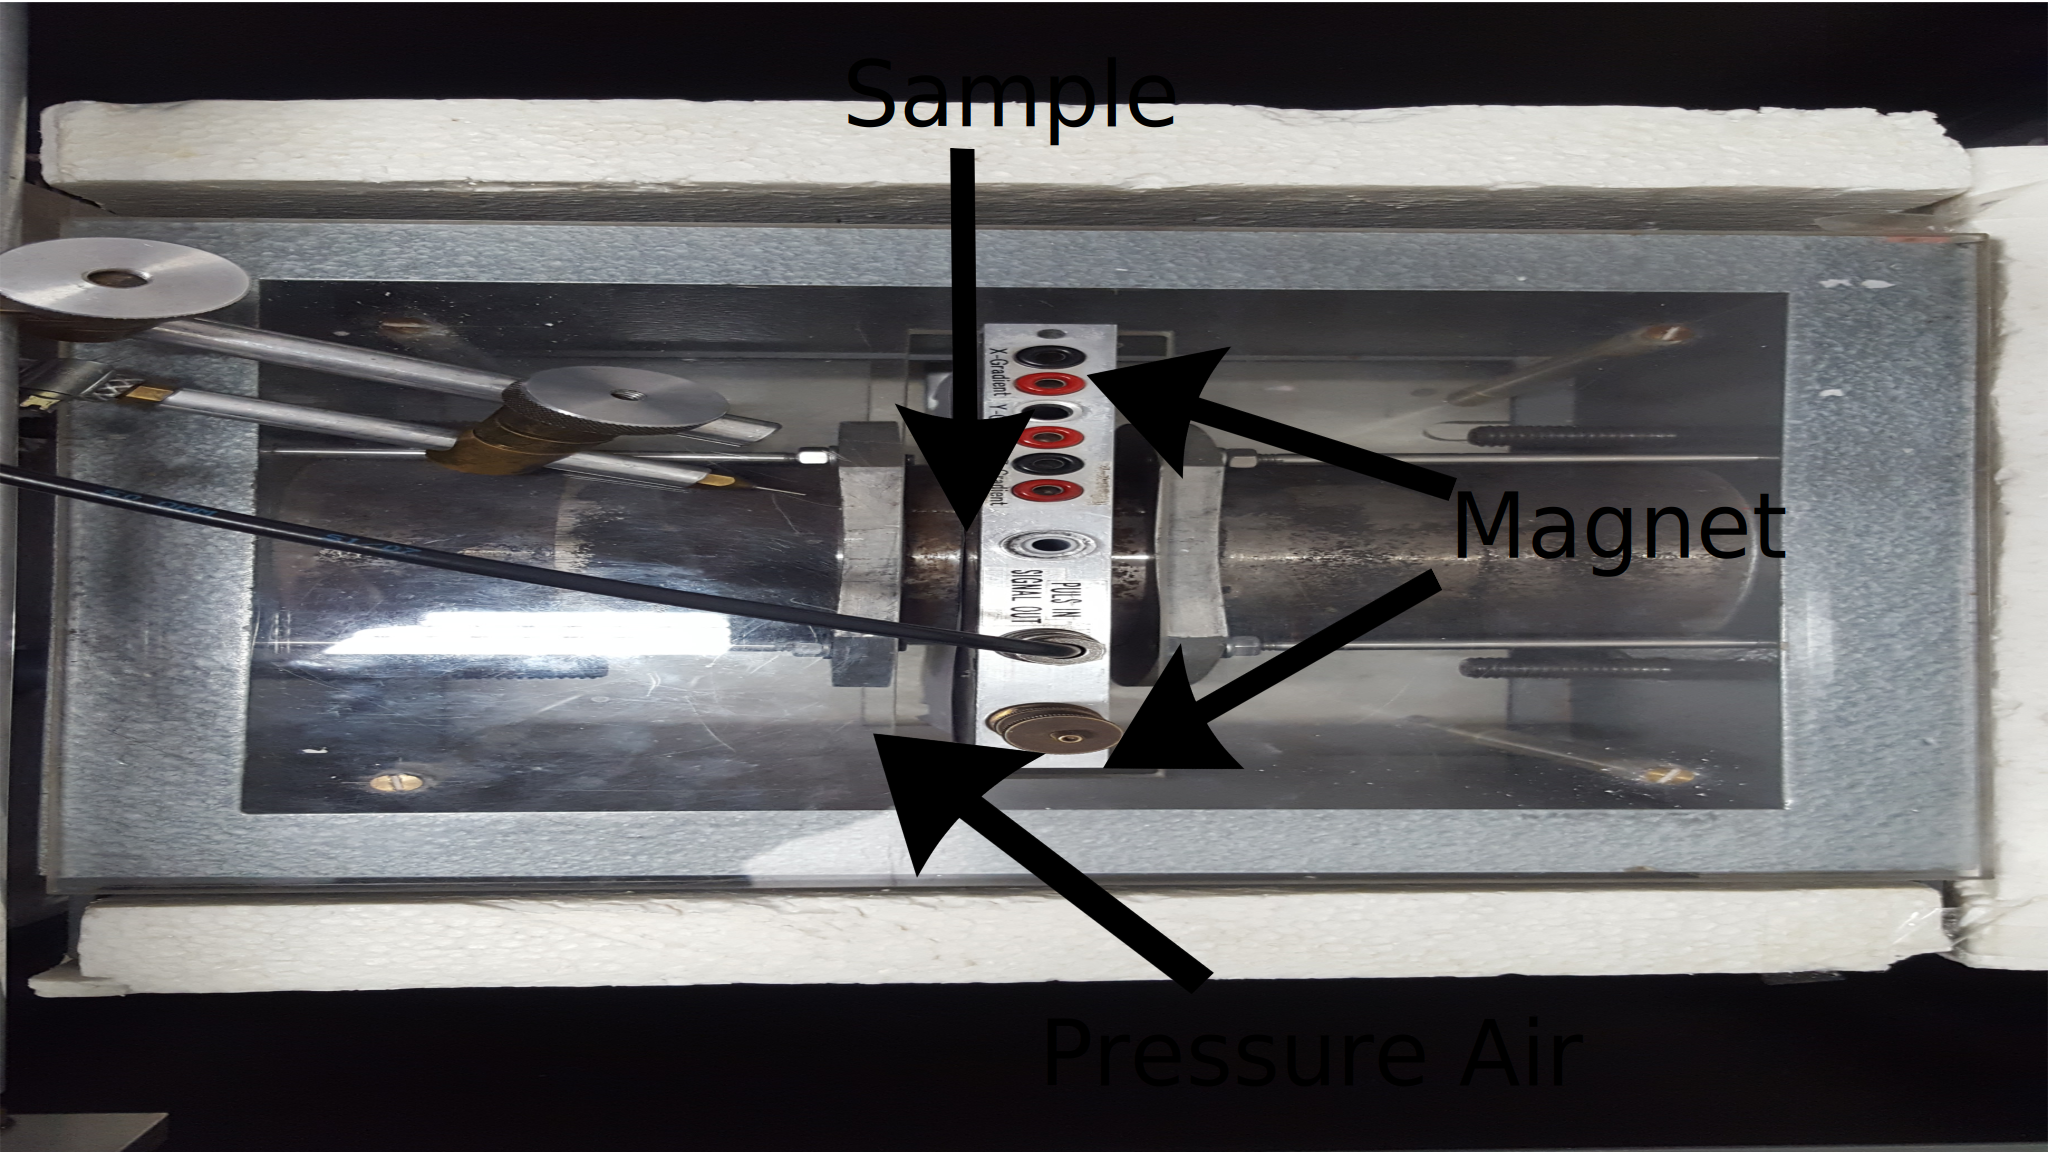
\includegraphics[scale=.075]{images//magnet.png}
	\caption{Magnet}
	\end{figure}
\end{frame}

\begin{frame}{Messung}
Messung der Spin-Spin Relaxationszeit $T_2$\\mit der Spin-Echo-Methode:
	\begin{figure}
	\centering
	% !TeX root = ..//fp_nmr_schmitt_kleinbek_18.tex
\begin{tikzpicture}[scale=.7]
%point
\foreach \i in {4.5,9}
\fill (\i,0) circle (2pt);

%circle
\foreach \i in {0,4.5,9,13.5}
\draw [thick] (\i,0) circle (1cm);

%time
\node at (0,2.5){$t=0$};
\node at (4.5,2.5){$t=\tau$};
\node at (9,2.5){$t=\tau$};
\node at (13.5,2.5){$t=2\tau$};
\node at (1.2,1.25)[color=grey]{$\ang{90}$-Puls};

%coordinates
\foreach \i in {0,4.5,9,13.5}
\draw[arrows=-{Stealth[scale=1]},thick](\i,0)--+(0,1.5) node[left]{$x$};
\foreach \i in {0,4.5,9,13.5}
\draw[arrows=-{Stealth[scale=1]},thick](\i,0)--+(1.5,0) node[below]{$y$};

%timearrows
\draw[arrows=-{Stealth[scale=.75]}, color=grey, line width=.75mm](2,0)--+(1,0) node[midway, above]{$\tau$};
\draw[arrows=-{Stealth[scale=.75]}, color=grey, line width=.75mm](6.5,0)--+(1,0) node[midway, above]{$\ang{180}$};
\draw[arrows=-{Stealth[scale=.75]}, color=grey, line width=.75mm](11,0)--+(1,0) node[midway, above]{$\tau$};

%arrows
\draw[arrows=-{Stealth[scale=.5]}, color=myred, line width=1.25mm](0,0)--+(1.2,0) node[midway, below, xshift=-3pt]{\footnotesize $M_\bot$};
\draw[arrows=-{Stealth[scale=.5]}, color=myred, line width=1.25mm](13.5,0)--+(-1.2,0) node[midway, below, xshift=3pt]{\footnotesize $M_\bot$};
\draw[arrows=-{Stealth[scale=1]},thick](4.5,0)--+(-35:1.5) node[below]{$\omega_2$};
\draw[arrows=-{Stealth[scale=1]},thick](4.5,0)--+(-60:1.5) node[below]{$\omega_1$};
\draw[arrows=-{Stealth[scale=1]},thick](9,0)--+(215:1.5) node[below]{$\omega_2$};
\draw[arrows=-{Stealth[scale=1]},thick](9,0)--+(240:1.5) node[below]{$\omega_1$};

\draw[arrows=-{Stealth[scale=1]},thick, shift = {(0.8,-0.8)}](5.42,-.4) arc (-25:-80:1);
\draw[arrows=-{Stealth[scale=1]},thick, shift = {(-0.8,-0.8)}](8.8,-.97) arc (-100:-155:1);

%redcircle
\foreach \i in {0,13.5}
\fill (\i,0) circle (1.775pt)[color=myred];
\end{tikzpicture}
	\caption{Spin-Echo-Methode}
	\end{figure}
\end{frame}

\begin{frame}{Messung}
	\begin{figure}
	\centering
	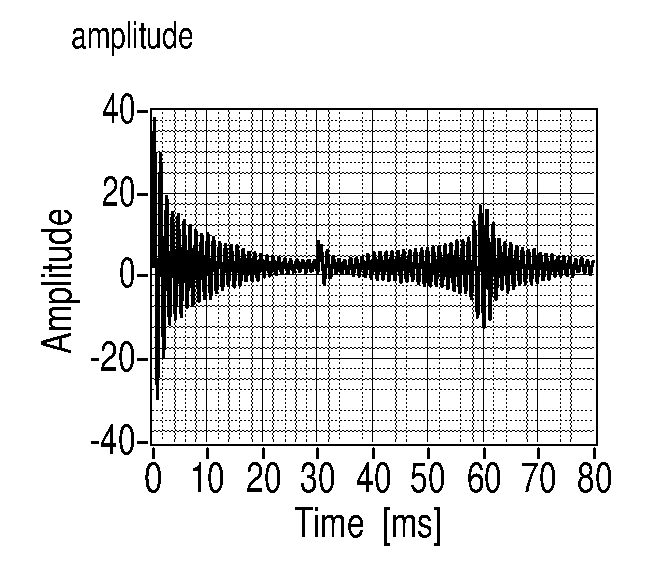
\includegraphics[width=7cm, height=4cm]{images//sequenz12.eps}
	\caption{Signal Spin-Echo-Methode}
	\end{figure}
\end{frame}

\begin{frame}{Messung}
Messung der Spin-Spin Relaxationszeit $T_2$\\mit der Carr-Purcell-Methode:
	\begin{align*}
	t =\begin{cases*} (2n+1)\tau: & \SI{180}{\degree} Puls \\ (2n)\tau: & kohärentes Signal \end{cases*}
	\end{align*}
	\begin{figure}
	\centering
	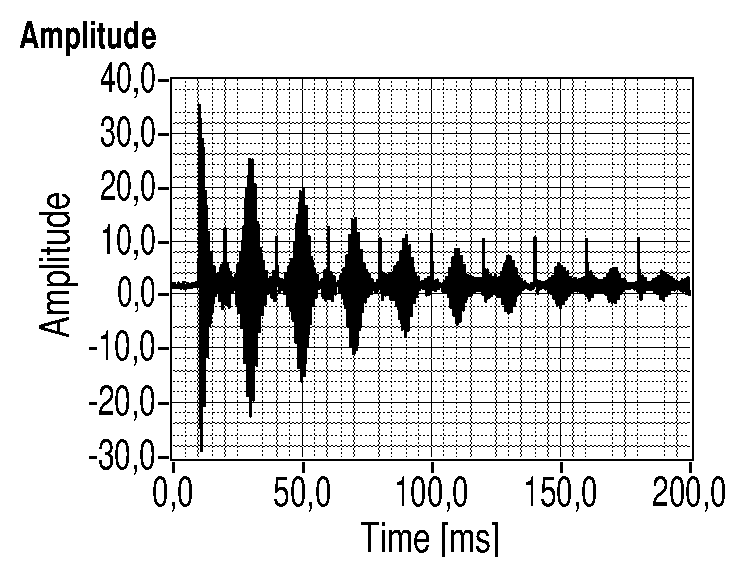
\includegraphics[width=7cm, height=4cm]{images//sequenzcp.eps}
	\caption{Signal Carr-Purcell-Methode}
	\end{figure}
\end{frame}

\begin{frame}{Messung}
	\begin{align*}
	M_\bot(t)&=M_0\cdot\e{-\frac{t}{T_2}}
	\end{align*}
	\begin{figure}
	\centering
		\begin{subfigure}{.49\textwidth}
		\centering
		\includegraphics[scale=.36]{..//figures//f61_abb_2.pdf}
		\caption{Spin-Echo}
		\end{subfigure}
		\begin{subfigure}{.49\textwidth}
		\centering
		\includegraphics[scale=.36]{..//figures//f61_abb_3.pdf}
		\caption{Carr-Purcell}
		\end{subfigure}
	\caption{Relaxationszeit $T_2$}
	\end{figure}
\end{frame}

\begin{frame}{Messung}
Messung der Spin-Gitter Relaxationszeit $T_1$:
\begin{itemize}
\item Drehung von $\vec{M}_\parallel$ mit \SI{90}{\degree} Puls nach $t=\tau$
\end{itemize}
	\begin{figure}
	\centering
	\begin{subfigure}{.49\textwidth}
	\centering
	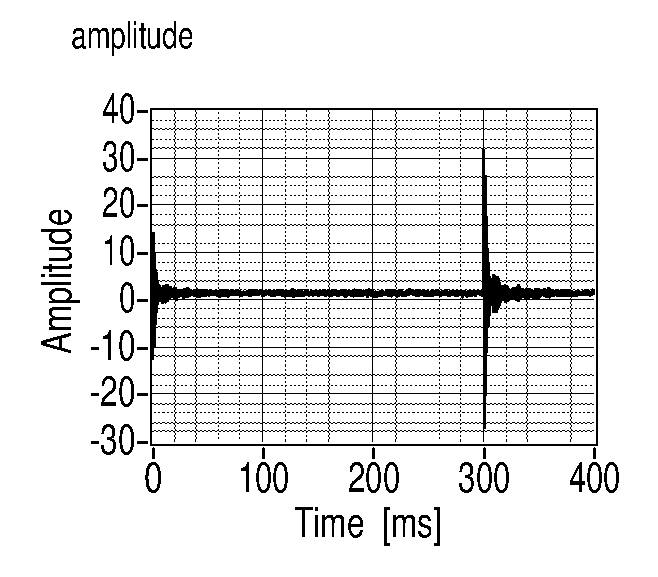
\includegraphics[width=5cm, height=3.6cm]{images//sequenz21.eps}
	\end{subfigure}
	\begin{subfigure}{.49\textwidth}
	\centering
	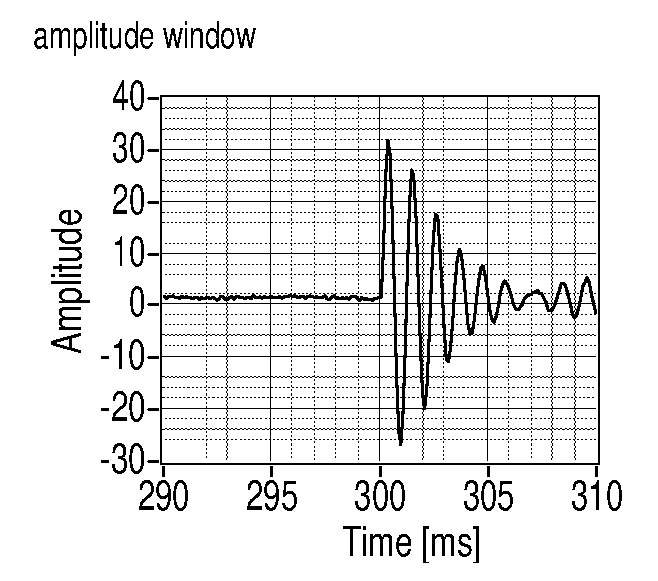
\includegraphics[width=5cm, height=3.6cm]{images//sequenz21einzel.eps}
	\end{subfigure}
	\caption{Spin-Gitter Relaxation}
	\end{figure}
\end{frame}

\begin{frame}{Messung}
Messung der Spin-Gitter Relaxationszeit $T_1$:
	\begin{align*}
	M_\parallel (t)&=M_0\left(1-2\cdot\e{-\frac{t}{T_1}}\right)
	\end{align*}
	\begin{figure}
	\centering
		\begin{subfigure}{.49\textwidth}
		\centering
		\includegraphics[scale=.36]{..//figures//f61_abb_1.pdf}
		\caption{Gd 500}
		\end{subfigure}
		\begin{subfigure}{.49\textwidth}
		\centering
		\includegraphics[scale=.36]{..//figures//f61_abb_1_600.pdf}
		\caption{Gd 600}
		\end{subfigure}
	\caption{Relaxationszeit $T_1$}
	\end{figure}
\end{frame}

\begin{frame}{Ergebnisse}
	\begin{table}
	\centering
	\begin{tabular}{cccc}
	\toprule
	Sample & $T_1$ [ms] & $T_{2,\text{ Spin-Echo}}$ [ms] & $T_{2,\text{ Carr-Purcell}}$ [ms]\\
	\midrule
	Gd500 & \num{190.0(6)} & \num{154.2(9)} & \num{170.1(4)}\\
	Gd600 & \num{234.3(5)} & \num{186.5(9)} & \num{198.2(7)}\\
	\bottomrule
	\end{tabular}
	\caption{Gemessene Relaxationszeiten}
	\end{table}
	\begin{block}{Schlussfolgerung}
	\begin{itemize}
	\item $T_\text{Spin-Echo} < T_\text{Carr-Purcell}$
	\item $T_2 < T_1$
	\item $T_\text{Gd500} < T_\text{Gd600}$	
	\end{itemize}
	\end{block}
\end{frame}




%---------------
%Chemical Shift
%---------------
\section{Chemische Verschiebung}

\begin{frame}{Physikalischer Hintergrund}
	\begin{itemize}
	\item Abschirmung durch Elektronen führt zu
	\begin{align*}
	\omega_i=\omega_\text{L}(1-\sigma_i)
	\end{align*}
	\end{itemize}
	\begin{block}{Abweichung zu Referenzstoff TMS}
	\[
	\delta_i=\frac{\omega_{TMS}-\omega_i}{\omega_\text{L}}
	\]
	\end{block}
	\begin{itemize}
	\item Messung des Frequenzspektrums\\
	$\Rightarrow$ Probe in Rotation versetzen
	\end{itemize}
\end{frame}

\begin{frame}{Messung}
\begin{figure}
	\centering
	\begin{subfigure}{.49\textwidth}
	\centering
	\includegraphics[scale=.36]{..//figures//f61_abb_6.pdf}
	\caption{mit TMS-Peak}
	\end{subfigure}
	\begin{subfigure}{.49\textwidth}
	\centering
	\includegraphics[scale=.36]{..//figures//f61_abb_6_ohne.pdf}
	\caption{ohne TMS}
	\end{subfigure}	
	\caption{Essigsäure}
	\end{figure}
\end{frame}

\begin{frame}{Physikalischer Hintergrund}
	\begin{figure}
	\centering
	\begin{subfigure}{.49\textwidth}
	\centering
	\includegraphics[width=5.4cm, height=4cm]{images//shift.png}
	\caption{$\delta_i$ relativ zu TMS}
	\end{subfigure}
	\begin{subfigure}{.49\textwidth}
	\centering
	\includegraphics[width=5cm, height=4cm]{images//substances.png}
	\caption{Verwendete Moleküle}
	\end{subfigure}	
	\caption{Chemische Verschiebung \cite{script_nmr}}
	\end{figure}
\end{frame}




%---------------
%Bildgebung
%---------------
\section{Bildgebende Verfahren} %2D- und 3D-Bildgebung
\begin{frame}{Physikalischer Hintergrund}
	\begin{itemize}
	\item Bildgebende Messverfahren benötigen $\vec{B}_0$ und Gradientenfelder:
	\begin{align*}
	\vec{B}_0&=(0,0,B_0)\\
	\vec{B}_x&=(0,0,G_x x)\\
	\vec{B}_y&=(0,0,G_y y)\\
	\vec{B}_z&=(0,0,G_z z)\\
	\end{align*}
	\item Mögliche Messmethoden:
		\begin{itemize}
		\item Frequenz Methode
		\item Phasen Methode
		\end{itemize}
	\end{itemize}
\end{frame}

\begin{frame}{Physikalischer Hintergrund}
Frequenz Methode:
	\begin{itemize}
	\item $\vec{M}_\bot$ wird durch $\operatorname{sinc}$ Puls generiert
	\item Einmaliges Einschalten des Gradientenfeld\\
	$\Rightarrow$ Ortsabhängige Larmorfrequenz $\omega_\text{L}$
	\end{itemize}
\vspace{.5cm}
Phasen Methode:
	\begin{itemize}
	\item $\vec{M}_\bot$ wird durch $\operatorname{sinc}$ Puls generiert
	\item Mehrmaliges Einschalten des Gradientenfeld\\
	$\Rightarrow$ Phasendifferenz der Kerne an unterschiedlichen Orten
	\end{itemize}
\end{frame}

\begin{frame}{Physikalischer Hintergrund}
Kombination von Phasen/Frequenz Methode für 2D %Hier vielleicht noch mehr Erklärungen auf die Folien
	\begin{figure}
	\centering
	\includegraphics[scale=.15]{images//signal.png}
	\caption{2D Bildgebung \cite{script_nmr}}
	\end{figure}
\end{frame}

\begin{frame}{Eindimensionale Messung}
	\begin{figure} %Bild von Reagenzglas mit Teflon, auch erklärung der Messungen auf Folien
	\centering
	\includegraphics[scale=.55]{..//figures//f61_abb_8.pdf}
	\caption{Öl in Reagenzglas}
	\end{figure}
\end{frame}

\begin{frame}{Eindimensionale Messung}
	\begin{figure} %Bild von Reagenzglas mit Teflon, auch erklärung der Messungen auf Folien
	\centering
	\begin{subfigure}{.49\textwidth}
	\centering
	\includegraphics[width=3cm, height=5cm]{images//oilteflon.jpg}
	\end{subfigure}
	\begin{subfigure}{.49\textwidth}
	\centering
	\makebox[\textwidth][c]{\includegraphics[width=1.2\textwidth]{..//figures//f61_abb_8_teflon.pdf}}
	\end{subfigure}
	\caption{Öl zwischen Teflon in Reagenzglas}
	\end{figure}
\end{frame}

\begin{frame}{Eindimensionale Messung}
Diffusionsgleichung: %Erklärung der Situation des Öls und Sands muss noch davor
	\begin{align*}
	\pdv{c(x,t)}{t}=D\pdv[2]{c(x,t)}{x}
	\end{align*}
	$\Rightarrow$ \enquote{zerlaufende} Gaußfunktion
	\begin{figure}
	\centering
	\includegraphics[scale=.4]{..//figures//gaus.pdf}
	\caption{Diffusionsprozess}
	\end{figure}
\end{frame}

\begin{frame}{Eindimensionale Messung}
	\begin{figure}
	\centering
	\includegraphics[scale=.35]{..//figures//f61_abb_9.pdf}
	\caption{Versickerungsprozess von Öl in Sand}
	\end{figure}
	\begin{block}{Schlussfolgerung}
	Diffusion spielt untergeordnete Rolle (Gravitation)
	\end{block}
\end{frame}

\begin{frame}{Zweidimensionale Messung}
	\begin{figure}
	\centering
	\includegraphics[scale=.5]{..//figures//chilipepper.png}
	\caption{Chilischote}
	\end{figure}
\end{frame}

\begin{frame}{Zweidimensionale Messung}
	\begin{figure}
	\centering
	\includegraphics[scale=.5]{..//figures//olive.png}
	\caption{Olive}
	\end{figure}
\end{frame}

\begin{frame}{Zweidimensionale Messung}
	\begin{figure}
	\centering
	\includegraphics[scale=.5]{..//figures//peanut.png}
	\caption{Erdnuss}
	\end{figure}
\end{frame}




%---------------
%Diskussion
%---------------
\section{Diskussion}
\begin{frame}{Anwendung}
Medizinischer Bereich
	\begin{figure}
	\centering
	\includegraphics[scale=.35]{images//mrt.jpg}
	\quelle{http://www.gesundmed.de/diagnose/magnet-resonanz-tomografie-mrt-kerspintomografie/}
	\caption{MRT}
	\end{figure}
\end{frame}

\begin{frame}{Fazit}
	\begin{alertblock}{-}
	\begin{itemize}
	\item Inhomogener Magnet ($\nicefrac{\Delta B}{B}\sim\num{e-5}$)
	\item Temperaturschwankungen
	\end{itemize}
	\end{alertblock}
	\begin{exampleblock}{+}
	\begin{itemize}
	\item Komponenten des ersten Messgeräts sind sichtbar
	\item Einblick in die 2D Bildgebung 
	\item Guten Einführung in einen Bereich der modernen Medizin
	\end{itemize}
	\end{exampleblock}
\end{frame}